\chapter{Programowanie ograniczeń}
\thispagestyle{chapterBeginStyle}

\section{Wprowadzenie}
    Programowanie ograniczeń (inna nazwa: technologia więzów) jest narzędziem wykorzystywanym do rozwiązywania 
    problemów z dziedzin kombinatoryki, sztucznej inteligencji, czy planowania jak i harmonogramowania zadań.
    W skład tego podejścia do programowania często wyróżnia się dwa elementy: ograniczenia (zwane również
    stałymi) oraz problem rozwiązywania ograniczeń (ang. Constraint Satisfaction Problem, CSP)
    Poniżej dokonano formalnego zdefiniowania powyższych komponentów:
    \begin{definition}
        \label{ConstraintProblem}
        \textbf{Problem rozwiązywania ograniczeń, CSP} jest następującą trójką:
        \begin{equation}
            CSP = (V,D,C)
        \end{equation}
        gdzie:

        $V = \{x_{1},x_{2},...,x_{n}\}$ oznacza zbiór zmiennych wykorzystywanych do opisu problemu

        $D = \{d_{1},d_{2},...,d_{n}\}$ oznacza zbiór dziedzin wyżej wspominanych zmiennych. W ramach 
        rozważań zawartych w rzeczonej pracy rozpatrywane będą takie $d_{i}$, które są zbiorami zawierającymi 
        skończoną liczbę potencjalnych wartości zmiennej $x_{i}$.

        $C = \{c_{1},c_{2},...,c_{m}\}$ oznacza zbiór ograniczeń
    \end{definition}
    \begin{definition}
        \label{Constraint}
        \textbf{Ograniczenami} (inne nazwy: stałe, więzy) nazywamy zmienne oraz zależności między nimi, które muszą zostać spełnione 
        w ramach rozwiązywania problemu ograniczeń. Określamy je przy pomocy pary: 
        \begin{equation}
            C = (S,R)
        \end{equation}
        gdzie:

        S jest krotką wszystkich zmiennych wchodzących w skład relacji 

        R jest relacją, która definiuje jakie wartości mogą przyjąc zmienne, które w niej uczestniczą.
    \end{definition}
    Relacje często przedstawia się przy pomocy zbioru zawierającego krotki, które składają się ze wszystkich 
    przyporządkowań wartości do odpowiednich zmiennych.
    Przy następujących definicjach oczekiwanym celem będzie utworzenie mechanizmu rozwiązującego zadany problem. Jego wynikiem 
    będzie zbiór wszystkich zmiennych, oraz krotek, które będą zawierały odpowiednie wartości przyporządkowane dla zmiennych.
    \begin{definition}
        \label{Krotka}
        \textbf{Krotka} (ang. tuple) - struktura danych, która w systemach informatycznych odzwierciedla uporządkowany ciąg wartości
    \end{definition}
    Dodatkowo wprowadza się termin \textbf{arności} ograniczenia:
    \begin{definition}
        \label{Krotka}
        \textbf{Arność ograniczenia} (ang. arity)  związana jest z liczbą unikalnych zmiennych, która w nią wchodzi.
    \end{definition}
    Najpopularniejszymi typami ograniczeń są:
    \begin{enumerate}
        \item Ograniczenia o arności 1, zwane ograniczeniami \textbf{unarnymi} (w tym przypadku z reguły będą one ściśle związane z dziedziną, raczej 
        nie będą występowały w kontekście ograniczeń)
        \item Ograniczenia o arności 2, zwane ograniczeniami \textbf{binarnymi}
        \item Ograniczenia o arności 3, zwane ograniczeniami \textbf{ternarnymi}
    \end{enumerate} 

    Tak jak ograniczenie może mieć swoją arność, tak dla CSP również zdefiniowano pojęcie arności w zmodyfikowany sposób 
    \begin{definition}
        \textbf{Arność} CSP o wartości $i$ zawiera w sobie wszystkie typy ograniczeń od arności 1 aż do arności $i$
    \end{definition}

    Wedle powyższego binarne CSP zawiera w sobie jedynie ograniczenia unarne jak i binarne.
    \begin{example}
        \label{CP1}
        Niech będzie dane równanie $x+y=z$, gdzie $x,y,z \in \{0,1\}$. Łatwo zauważyć, iż zadane równanie jest automatycznie ograniczeniem 
        wpływającym na prezentowane zmienne. Przyporządkowując odpowiednie wartości do zbiorów z definicji \label{ConstraintProblem} otrzymano
        \begin{enumerate}
            \item $ V = \{x,y,z\} $
            \item $ D = \{d_{x},d_{y},d_{z}\}$, gdzie $d_{x},d_{y},d_{z} = \{0,1\}$
            \item $ C = \{x+y=z\}$
        \end{enumerate}
        \textbf{Arność} ograniczenia występujące w przedstawionym przykładzie wynosi 3, determinowane jest to liczbą zmiennych, która wchodzi w jej skład.
        Rozwiązaniem tego problemu będą następujące dopasowania:

        
        $((x,y,z),\{0,0,0\}, \{1,0,1\}, \{0,1,1\})$

    \end{example}
    Odnalezienie rozwiązań z przykładu \ref{CP1} było trywialne ze względu na małą liczbę zmiennych, wąskie dziedziny oraz tylko jedno wprowadzone ograniczenie.
    Podobnie jak z planowaniem, wprowadzenie dodatkowych zmiennych, powiększanie dziedzin oraz zbioru ograniczeń znacznie wpływa na skomplikowanie 
    odnajdowania rozwiązania.



\section{Pojęcie ustalenia i spójności}
    \label{SpójnośćRodział}
    W ostatecznej formie problem ograniczeń wyszukuje rozwiązanie przy pomocy ustalenia wartości zmiennych, jednakże najistotniejsza 
    jest droga, jaką pokonuje, aby ów ustalenia uzyskać. W tej sekcji należy wprowadzić kilka dodatkowych definicji:
    \begin{definition}
        Ustalenie zmiennych jest \textbf{spójne}, gdy nie jest w konflikcie z żadnym z ograniczeń.
    \end{definition}
    Ustalenie spójne również w nomenlakturze programowania ograniczeń nazywane jest ustaleniem \textbf{legalnym}.
    Nadanie zmiennym X oraz Y wartość 1 w przykładzie \ref{CP1} prowadzi do konfliktu, gdyż nie istnieje wartość 2 w zbiorze $D_{z}$.
    \begin{definition}
        \textbf{Kompletnym ustaleniem} nazywamy takie ustalenie, w którym wszystkie zmienne posiadają ustaloną wartość.
    \end{definition}
    Łatwo zauważyć, iż kompletne ustawienie jest jednocześnie rozwiązaniem problemu ograniczeń. Z tego płynie następujący wniosek:
    \begin{corollary}
        Każde rozwiązanie problemu ograniczeń jest spójne.
    \end{corollary}

    Dodatkowo definiuje się częściowe ustalenie oraz częściowe rozwiązanie \cite{AI}. Zgodnie \\
    z nazewnictwem 
    częściowe ustalenie związane jest z sytuacją, gdy nie wszystkie zmienne mają dokładnie określone wartości, natomiast 
    częściowe rozwiązanie w praktyce identyfikuje się jako spójne częściowe ustalenie.

    Po wprowadzeniu powyższych definicji należy rozpocząć rozważania na temat tego, w jaki sposób 
    problem ograniczeń może zostać rozwiązany. Pierwszym z podejść może być ustalenie wartości dla zmiennych poprzez 
    analizę ograniczeń, jakie między nimi występują. Ten proces nazywany jest \textbf{propagacją ograniczenia}. Dzięki 
    podstawowej analizie ograniczeń algorytm może wyeliminować wartości nadmiarowe znajdujące się w zadanych dziedzinach, co znacząco wpłynie 
    na przyszłościowe osiągi pod kątem czasowym. Często propagacja ograniczeń jest wykonywana jako \textit{preprocessing step}, czyli 
    jako krok, który zostanie wykonany jeszcze przed rozpoczęciem prawdziwej pracy nad problem. 
    
    Przy rozwiązywaniu problemów związanych z ograniczeniami bardzo intuicyjną reprezentacją, jest reprezentacja 
    w formie \textit{grafu}. Poprzez wierzchołki oznacza się zmienne wchodzące w skład problemu, natomiast poprzez krawędzie- 
    binarne ograniczenia, która między nimi występują. Z tego powodu pożądanym zabiegiem będzie przedstawienie wszystkich ograniczeń 
    n-arnych w formie binarnej.

    Kluczem do uzyskania poprawnego efektu propagacji ograniczeń jest skorzystanie z pojęcia zdefiniowanego jako \textbf{lokalna spójność}.
    Istnieją różne typy lokalnej spójności:
    \begin{itemize}
        \item \textbf{Spójność wierzchołkowa} (ang. node consistency) - Zmienna jest wierzchołkowo spójna, 
        gdy wszystkie wartości znajdujące się w jej dziedzine spełniają zdefiniowane przez nią ograniczenie unarne.
        Graf jest wierzchołkowo spójny, gdy wszystkie wierzchołki wchodzące w skład grafu są wierzchołkowo spójne.
        Zachowanie wierzchołkowej spójności \\
        z reguły sprowadza się do \textbf{zawężania} dziedziny zmiennej.
        \item \textbf{Spójność krawędziowa} (ang. arc consistency/edge consistency)- Zmienna jest spójna krawędziowo wtedy, 
        gdy każda wartość z jej dziedziny spełnia binarne ograniczenia zmiennej. Graf jest krawędziowo spójny gdy każda para 
        zmiennych jest ze sobą krawędziowo spójna.
        \item \textbf{Spójność ścieżki} (ang. path consistency) - Dwie zmienne $a,b$ są spójne w kontekście ścieżki z trzecią zmienną 
        $c$, gdy każde przypisanie wartości do zmiennych $a,b$ spełniające ograniczenie występujące między rzeczonymi zmiennymi dodatkowo 
        spełnia ograniczenie między zmiennymi $a,c$ oraz $c,b$.
        \item \textbf{K-spójność}- CSP jest k-spójne, gdy dla każdego spójnego ustalenia zawierającego $k-1$ zmiennych można dołączyć k-tą zmienną 
        bez załamiania spóności. Pojęcie 2-spójność jest tożsame z spójnością krawędziową, a 3-spójność- ze spójnością ścieżki.
    \end{itemize}

    Sprowadzanie problemu ograniczeń do sytuacji, w której zachodzi lokalna spójność jest określane mianem \textbf{propagacji ograniczeń}. 
    Jest to o tyle istotne, iż jedną z głównych metod rozwiązywania problemu ograniczeń jest sprowadzenie, o ile to możliwe, dziedzin zmiennych do pojedynczej wartości- 
    wtedy całkowitym ustaleniem jest nadanie zmiennej jedynej wartości w swojej dziedzinie. Propagacja ograniczeń jest silnym mechanizmem wykrywającym 
    niespójności- jeśli przy próbie propagacji któraś z wartości zostałaby z pustą dziedziną, wtedy należałoby przerwać rozwiązywanie problemu wraz 
    ze zwróceniem informacji o fakcie, iż nie ma takiego ustalenia zmiennych przy obecnych dziedzinach, dla którego rozpatrywane ograniczenie 
    jest rozwiązywalne.

\section{Ograniczenia globalne}
    W teorii programowania ograniczeń istnieją również ograniczenia zwane \textbf{globalnymi} \cite{CP}. Mimo swojej nazwy, 
    globalne ograniczenia nie zawsze są związane ze wszystkimi zmiennymi wchodzącymi w skład problemu ograniczeń. 
    Ich istnienie warunkowane jest występowaniem w świecie rzeczywistym zależności, które często się powtarzają i nie są 
    unikalne dla jednego problemu. Przykładem takiego ograniczenia jest sytuacja, w której każda ze zmiennych ma mieć inną wartość.
    Formalniej mówiąc, wszystkie zmienne muszą być parami różne. Ograniczenie to jest na tyle popularne, iż nosi ono swoją nazwę 
    \textbf{Alldiff} i jest często ograniczeniem wbudowanym w moduły zajmujące się programowaniem ograniczeń, co ułatwia i przyśpiesza 
    pracę użytkownika. Innym ograniczeniem z rodziny ograniczeń globalnych jest \textbf{ograniczenie zasobów}. Jak sama nazwa wskazuje, 
    rzeczone ograniczenie globalne wykorzystywane jest w modelowaniu sytuacji z dziedzin planowania bądź harmonogramowania zadań. 
    Przy rozwiązywaniu tego typu ograniczenia częstą metodą jest sumowanie wartości zmiennych wchodzących w skład dziedziny \cite{AI}.
    
    
\section{Wyszukiwanie rozwiązań}
    Podstawową metodą rozwiązywania problemów z dziedziny ograniczeń nosi miano metody \textbf{cofającej}, bądź też programowania wstecz (ang. backtracking).
    Działa ona zbliżenie do mechanizmu przeszukiwania grafu wgłąb. Na początku wybierana jest jedna ze zmiennych. Dla każdej wartości 
    z dziedziny dochodzi do częściowego ustalenia- zmienna otrzymuje wartość równą pierwszej wartości w swojej dziedzinie. Następnie, 
    korzystając z tej informacji dochodzi do propagacji ograniczeń. Jeśli wybrana została poprawna wartość propagacja ograniczeń doprowadzi 
    do znalezienia rozwiązania problemu. Istnieje również sytuacja, w której wybrana wartość prowadzi do slepego zaułka, czyli do sytuacji, w której 
    nie istnieje odpowiednie ustalenie zmiennych. Wtedy należy \textbf{cofnąć} 
    się do miejsca, w którym zmiennej nadaliśmy wartość i spróbować innego ustalenia. 
    Połączenie mechanizmu cofnięcia wraz z propagacją ograniczeń, czyli z utrzymywaniem lokalnej spójności na każdym etapie 
    wyszukiwania rozwiązania jest znakomitą techniką poprawiającą wydajność. Dzięki propagacji ograniczeń często 
    dochodzi do sytuacji, w której wyżej wymienione ślepe zaułki są eliminowane zanim mechanizm cofania je rozpatrzy. 
    
    Drugą metodą jest metoda nazywana \textbf{wyszukiwaniem lokalnym} (ang. local search). Metoda cofająca, jak sama nazwa wskazuje, próbowała dokonać 
    częściowego ustalenia, \\
    aby następnie przy propagacji ograniczeń udowodnić, iż rozpatrywane częściowe ustalenie jest prawidłowe 
    i wygenerować odpowiednie całkowite ustalenie. Metodologia wyszukiwania lokalnego różni się w swojej filozofii tym, iż na samym 
    początku dochodzi do pełnego ustalenia zmiennych. W znacznej większości przypadków pełne ustalenie jest 
    nieprawidłowe, to znaczy nie spełnia wszystkich ograniczeń. Wtedy mechanizm próbuje na bieżąco naprawiać sytuację modyfikując całkowite ustalenie w taki 
    sposób, aby ustalenie nadal było całkowite jednocześnie spełniając ograniczenie, które wcześniej powodowało konflikty. Jeśli algorytm będzie
    w stanie 
    rozwiązać wszystkie ograniczenia uzyska odpowiednie ustalenie zmiennych.

    Porównując powyższe dwie metody łatwo zauważyć, iż różnią się one od siebie w znacznym stopniu, nie tylko w samej filozofii działania, lecz także 
    w efektach.

    \begin{definition}
        \label{AlgorytmKompletny}
        \textbf{Algorytmem kompletnym} jest algorytm, który gwarantuje uzyskanie rozwiązania oraz jest w stanie 
        wykryć, gdy takowe rozwiązanie nie istnieje
    \end{definition}

    Przeciwieństwem algorytmu kompletnego jest algorytm \textbf{niekompletny}, czyli taki, który nie gwarantuje 
    uzyskania optymalnego rozwiązania oraz wykrycia, czy problem posiada rozwiązanie. Algorytmy niekompletne natomiast są o wiele 
    szybsze oraz dla wielu przypadków dobrze przybliżają optymalne rozwiązanie. 

    Zgodnie z powyższym metoda cofająca jest przykładem algorytmu kompletnego- systematycznie generuje nowe ustalenia oraz propagacje ograniczeń,
    natomiast wyszukiwanie lokalne jest przykładem algorytmu niekompletnego- łatwo sobie wyobrazić sytuację nierozwiązywalną, dla której naprawienie jednego ograniczenia 
    może nieustannie generować zepsucie kolejnego. Dla takiej sytuacji algorytm będzie próbował w nieskończoność przestawiać elementy, 
    nie wiedząc o tym, iż poprawne ustawienie nie istnieje.W trakcie wyboru algorytmu ważnym jest, aby znać jego zalety jak i wady. Do implementacji 
    GRAPHPLANU został wykorzystany mechanizm cofania, aby zwracany przez algorytm plan był zawsze optymalny.

    Powyżej wymienione metody posiadają wiele dodatkowych usprawnień oraz specjalnie zdefiniowanych heurystyk. \cite{CP}
    
\section{Programowanie w logice z ograniczeniami}
    Ze względu na wiele podobieństw w mechanizmach, jak i w samej idei, między technologią więzów a programowaniem w logice, takich jak chociażby mechanizm cofania, który jest 
    powszechnie wykorzystywany w obu podejściach, zdecydowano się na utworzenie połączenia między nimi w celu uzyskania korzystniejszych wyników. Z tej kombinacji powstał 
    typ programowania nazywany \textbf{Programowaniem w logice z ograniczeniami}.
    \begin{definition}
        \textbf{Programowanie w logice z ograniczeniami} (ang. Constraint logic programming) jest jedną z form programowania,
        w której podstawowe mechanizmy programowania w logice zostały rozszerzone o koncpecje pochodzące z programowania ograniczeń.
    \end{definition}

    \begin{example}
        Programowanie ograniczeń zastosowane w języku PROLOG, który jest językiem programowania logicznego:
        \begin{listing}[H]
            \begin{minted}{prolog}
                FUNC(X,Y) :-
                X+Y > 0,
                writeln(X),
                wirteln(Y).
            \end{minted}
            \caption{Metoda wypisująca liczby gdy ich suma jest większa od 0}
        \end{listing}
    \end{example}
    W powyższym przykładzie zastosowano najprostsze z możliwych ograniczeń: wartość sumy zmiennych musi być większa od 0. 
    Ze względu na częste parowanie programowania ograniczeń z programowaniem w logice, wiele implementacji języków logicznych zawiera
    gotowe moduły, które dostarczają technologię więzów dla różnych typów dziedzin. Dla
    jednej z najpopularniejszych implementacji języka programowania PROLOG dostępne są następujące moduły:
    \begin{itemize}
        \item \textbf{clpfd} -- moduł, w którym dziedziny są skończone i składają się z liczb całkowitych. \\
        Ów moduł 
        wykorzystywany jest w zaimplementowanym algorytmie GRAPHPLAN
        \item \textbf{clpb} -- moduł, w którym dziedziny składają się z wartości boolowskich
        \item \textbf{clpq} -- moduł, w którym dziedziny składają się z liczb wymiernych w formie dziesiętnej
        \item \textbf{clpr} -- moduł, w którym dziedziny składają się z liczb rzeczywistych zmiennopozycyjnych 
    \end{itemize}
    Dzięki powyższym modułom można tworzyć bardziej zmyślne ograniczenia. Z przykładami takich zastosowań
    czytelnik będzie mógł się zapoznać w sekcji opisującej implementację algorytmu.

\section{Obrazowe przykłady}
    \subsection{Problem plecakowy}
    Przykładem realizacji problemu ograniczeń poprzez wykonanie operacji propagacji ograniczeń wraz z mechanizmem cofania będzie popularny \textbf{Problem plecakowy}
    \begin{example}
        \textbf{Dyskretny problem plecakowy}- (ang. discrete knapsack problem) problem wyboru przedmiotów w taki sposób, aby spełniały następujące założenia:
        \begin{itemize}
            \item suma wartości wybranych przedmiotów musi być jak największa 
            \item suma wag wybranych przedmiotów nie może przekraczać pojemności plecaka
        \end{itemize}
    \end{example}

    Pierwszym podejściem, automatycznie nasuwającym się przy próbie rozwiązania tego problemu, 
    jest itercyjne pakowanie przedmiotów o najwyżej wartości aż do zajścia
    sytuacji, \\
    w której plecak nie jest w stanie pomieścić następnego przedmiotu lub nie ma więcej przedmiotów wskazanego typu. 
    Wtedy dochodzi do zmiany przedmiotu na ten, który jest 
    drugi co do wartości oraz powtórzenia dla niego wyżej opisanego procesu. Łatwo zauważyć, iż takie rozwiązanie, mimo tego, że zawsze wyprodukuje 
    wynik, jest mało optymalne. Mogą zdarzyć się sytuacje, w których przedmiot o dużej wartości jest na tyle ciężki, że warto byłoby z niego 
    zrezygnować na rzecz mniej wartościowych, ale za to lżejszych przedmiotów. Takie sytuacje nie zostaną wychwycone przez takowe podejście. 
    Przedstawiony powyżej sposób rozwiązania problemu nosi nazwę rozwiązania \textbf{zachłannego}, które cechuje się wyszukiwaniem lokalnego, a
    nie globalnego, \textbf{ekstremum} funkcji.

    Łatwo zauważyć, iż sposób zachłanny jest modelowany na wzór zachowania człowieka postawionego we wskazanej sytuacji. Drugie podejście natomiast 
    wykorzystuje analityczne podejście, które w świecie informatycznym nosi nazwę \textbf{programowania dynamicznego}. Ten typ programowania 
    opiera się na podziale występującego problemu na mniejsze podproblemy względem ustalonych parametrów. Dla wskazanego problemu 
    definiuje się ciąg wag jako $w_{1},...,w_{n}$ oraz wartości $v_{1},...,v_{n}$, gdzie \textbf{n} oznacza liczbę branych pod uwagę przedmiotów, 
    oraz funkcję $A(i,j)$, gdzie \textbf{i} oznacza liczbę rozpatrzonych już elementów, a \textbf{j}- maksymalną wartość, którą można otrzymać ze wskazanych 
    elementów. Problem sprowadza się do wyznaczenia wartości $A(n,W)$, gdzie \textbf{W} oznacza maksymalną wagę plecaka.
    Funkcja $A(i,j)$ definiowana jest następującym wzorem:
    \begin{gather}
        \nonumber A(0,j) = 0 \\
        \nonumber A(i,0) = 0 \\
        \nonumber A(i,j) = A(i-1,j) : w_{i} > j\\
        A(i,j) = max(A(i-1,j), A(i-1,j-w_{i}) + v_{i}) : w_{i} \leq j
    \end{gather}
    Funkcja ta nosi nazwę \textit{funkcji rekurencyjnej Bellman'a}


    Alternatywną metoda do skomplikowanego podejścia w programowaniu dynamicznym jest użycie wcześniej wspomnianego programowania ograniczeń.
    Ograniczenie na liczbę przedmiotów prezentowane jest w postaci $w_{1}*A + w_{2}*B + ... =< W$, gdzie współczyniki $A,B,...$ \\
    to liczba elementów do wzięcia.
    Następnie należy zmaksymalizować etykietowanie współczynników $A,B,...$ względem funkcji $v_{1} * A + v_{2} * B + ...$.


    \subsection{Krypto-arytmetyczna łamigłówka}
    Krypto-arytmetyczna łamigłówka jest przykładem matematycznego równania, w którym cyfry zastąpiono przez litery. Zadaniem rozwiązującego 
    jest zamiana odpowiednich liter na cyfry w taki sposób, aby prezentowane równanie było matematycznie poprawne.
    \begin{example}
        \begin{figure}[H]
            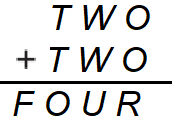
\includegraphics[scale=0.5]{constraint_example}
            \centering
            \caption{Przykładowa łamigłówka krypto-arytmetyczna \cite{AI}}
        \end{figure} 
    \end{example}
    Najważniejszymi założeniami łamigłówki są:
    \begin{itemize}
        \item Wartości ukryte pod literami T,W,O,F,U,R są parami różne
        \item Najbardziej znacząca cyfra jest niezerowa (w tym przypadku $T \neq 0 $ oraz $F \neq 0$)
    \end{itemize}

    Pierwszy sposób na rozwiązanie, bez użycia programowania ograniczeń:

    \begin{listing}[H]
        \begin{minted}{prolog}
        digit(0). digit(1). digit(2). digit(3). digit(4).
        digit(5). digit(6). digit(7). digit(8). digit(9).

        riddle([T,W,O],[T,W,O],[F,O,U,R]) :-
            digit(T), digit(W), digit(O),
            digit(F), digit(U), digit(R),
            T =\= W, T =\= O, T =\= F, T =\= U, T =\= R,
            W =\= T, W =\= O, W =\= F, W =\= U, W =\= R, 
            O =\= T, O =\= W, O =\= F, O =\= U, O =\= R,
            F =\= T, F =\= W, F =\= O, F =\= U, F =\= R,
            U =\= T, U =\= W, U =\= O, U =\= F, U =\= R,  
            R =\= T, R =\= W, R =\= O, R =\= F, R =\= U,
            T > 0, F > 0,
            100*T + 10*W + O + 100*T + 10*W + O  =:= 1000*F + 100*O + 10*U + R. 
        \end{minted}
    \caption{Implementacja rozwiązania łamigłówki krypto-arytmetycznej bez użycia programowania ograniczeń}
    \end{listing}

    Drugi sposób na rozwiązanie problemu, z użyciem programowania ograniczeń:

    \begin{listing}[H]
        \begin{minted}{prolog}
        :- use_module(library(clpfd)).

        riddle([T,W,O],[T,W,O],[F,O,U,R]) :-
            Values = [T,W,O,F,U,R],
            Values ins 0..9,
            all_different(Values),
            T #> 0,
            F #> 0,
            100*T + 10*W + O + 100*T + 10*W + O #= 1000*F + 100*O + 10*U + R,
            label(Values).
        \end{minted}
    \caption{Implementacja rozwiązania łamigłówki krypto-arytmetycznej z użyciem programowania ograniczeń}
    \end{listing}

    Otrzymane przykładowe rozwiązanie $T=7, W=3, O=4, F=1, U=6, R=8$.

    \begin{figure}[H]
        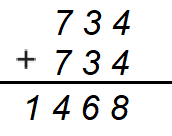
\includegraphics[scale=0.5]{constraint_example_solved}
        \centering
        \caption{Przykładowe rozwiązanie wskazanej łamigłówki}
    \end{figure} 

    Porównanie osiągnięc wskazanych rozwiązań:
    
    \begin{table}[H]
        \centering
         \begin{tabular}{||c | c | c||} 
         \hline
         Sposób & Wnioskowania & Czas[s] \\ [0.5ex] 
         \hline\hline
         Bez CLP & 8 679 856 & 0.449 \\ 
         \hline
         Z CLP & 19 119 & 0.002  \\ [1ex]
         \hline
         \end{tabular}
         \caption{Otrzymane wyniki dla znalezienia pierwszego rozwiązania łamigłówki}
    \end{table}

\section{Wykorzystanie w algorytmie}

    Podczas opisywania mechanizmów stojących za programowaniem ograniczeń często wykorzystywaną strukturą był graf, chociażby w sekcji omawiającej 
    pojęcie lokalnych spójności (\ref{SpójnośćRodział}). Ze względu na ów powiązanie między programowaniem ograniczeń a GRAPHPLAN'em do podstawowego opisu GRAPHPLAN'u z rodziału 
    \ref{GRAPHPLANRozdzial} dodano funkcjonalności opisane w powyższych rozdziałach. 

    Każdy ze stanów oraz akcji zawiera w sobie dodatkowy \textbf{indykator}. Jest to liczba ze zbioru liczb całkowitych, o której 
    należy mysleć bardziej w kontekście wartości bool'owskich $\{prawda,fałsz\}$. Wartość liczby równa 0 jest równoważna fałszywość stanu, natomiast wartość większa od 0 generuje jego
    prawdziwość. Przy pomocy indykatorów program ustala, które stany, bądź akcje 
    są w danej warstwie prawdziwe, czyli występują w świecie oraz takie, które
    w ów świecie w danym momencie nie występują, czyli są fałszywe. 
    Odbywa się to w następujący sposób:
    \begin{enumerate}
        \item Wszystkie stany wchodzące w stan początkowy otrzymują indykator równy 1, gdyż są aktualnie prawdziwe 
        w rozpatrywanym świecie.
        \item W trakcie generowania akcji następuje utworzenie powiązania między warunkami zajścia, akcjami oraz ich efektami.
        Akcja zostaje powiązana ze swoim warunkiem następującym ograniczeniem: wartośc indykatora akcji jest mniejsza bądź równa wartości 
        indykatora warunku. Należy to rozumieć w następujący sposób- jeśli warunek jest prawdziwy to akcja \textbf{może} zachodzić w świecie, natomiast 
        jeśli warunek jest nieprawdziwy, czyli ma indykator równy 0, akcja automatycznie dostaje indykator równy 0.
        Efekt zostaje powiązany ze swoją akcją poprzez następujące ograniczenie: jeśli jakakolwiek akcja w danej warstwie, 
        która ma dany stan za efekt, zachodzi, wtedy również i efekt w nim występuje. Jeśli wszystkie akcje generujące ów efekt mają indykator równy 0 
        wtedy efekt nie może zachodzić na danym poziomie, więc również otrzymuje indykator równy 0.
        \item Dochodzi do sprawdzenia relacji wzajemnego wykluczania poprzez sprawdzenie indykatorów dwóch stanów- Jeśli ich iloczyn jest równy 0, wtedy 
        dwa stany nie mogą razem występować na danym poziomie.
        \item Przy dokładnej realizacji kroków 2 i 3 algorytm jest w stanie wygenerować kolejny poziom stanów. Po wygenerowaniu 
        dochodzi do sprawdzenia, czy istnieje takie ustalenie wartości ograniczeń na stanach zawartych w danej warstwie algorytmu, aby wszystkie 
        stany wchodzące w zbiór celów otrzymały indyaktor równy 1. Jeśli nie, 
        rzeczony proces jest powtarzany aż do otrzymania pożądanego skutku.
        \item Gdy wszystkie cele otrzymają indykator 1, program przelicza wszystkie indykatory, dzięki czemu jest w stanie bezbłędnie określić, który 
        stan bądź która akcja na danym etapie przetwarzania świata znajdują się w nim bądź nie. Ów mechanizm jest silnie wykorzystywany 
        przy generowaniu grafów, przedstawiających zachodzące w świecie zmiany.
    \end{enumerate}

    Dzięki tej z pozoru niewielkiej modyfikacji algorytmu GRAPHPLAN zyskuje on zdecydowane przyśpieszenie w fazie kreowania planu. Gdy GRAPHPLAN dojdzie do odpowiedniego
    poziomu stanów, gdzie znajdują się wszystkie stany ze zbioru celów, wszystkie komponenty wchodzące w skład grafu planującego będą miały dodatkową informację o swojej prawdziwości 
    w danej warstwie. Odnalezienie planu sprowadza się do rozwiązania problemu ograniczeń dla wszystkich stanów grafu. Dokonywane jest to wedle myśli przewodniej GRAPHPLANU, czyli 
    poprzez mechanizm cofania wraz z propagacją ograniczenia przy zachowaniu lokalnej spójności. Bez tej modyfikacja wyłuskanie planu z grafu planującego przypominałoby wyszukiwanie 
    w głąb w grafie. Przechowywanie dodatkowej informacji w formie indykatora znacznie usprawnia ten proces.

    Dokładne sformuowanie ograniczeń przy pomocy symboli matematycznych odbędzie się w sekcji poświęconej implementacji algorytmu.
    